
% Default to the notebook output style

    


% Inherit from the specified cell style.




    
\documentclass[11pt]{article}

    
    
    \usepackage[T1]{fontenc}
    % Nicer default font (+ math font) than Computer Modern for most use cases
    \usepackage{mathpazo}

    % Basic figure setup, for now with no caption control since it's done
    % automatically by Pandoc (which extracts ![](path) syntax from Markdown).
    \usepackage{graphicx}
    % We will generate all images so they have a width \maxwidth. This means
    % that they will get their normal width if they fit onto the page, but
    % are scaled down if they would overflow the margins.
    \makeatletter
    \def\maxwidth{\ifdim\Gin@nat@width>\linewidth\linewidth
    \else\Gin@nat@width\fi}
    \makeatother
    \let\Oldincludegraphics\includegraphics
    % Set max figure width to be 80% of text width, for now hardcoded.
    \renewcommand{\includegraphics}[1]{\Oldincludegraphics[width=.8\maxwidth]{#1}}
    % Ensure that by default, figures have no caption (until we provide a
    % proper Figure object with a Caption API and a way to capture that
    % in the conversion process - todo).
    \usepackage{caption}
    \DeclareCaptionLabelFormat{nolabel}{}
    \captionsetup{labelformat=nolabel}

    \usepackage{adjustbox} % Used to constrain images to a maximum size 
    \usepackage{xcolor} % Allow colors to be defined
    \usepackage{enumerate} % Needed for markdown enumerations to work
    \usepackage{geometry} % Used to adjust the document margins
    \usepackage{amsmath} % Equations
    \usepackage{amssymb} % Equations
    \usepackage{textcomp} % defines textquotesingle
    % Hack from http://tex.stackexchange.com/a/47451/13684:
    \AtBeginDocument{%
        \def\PYZsq{\textquotesingle}% Upright quotes in Pygmentized code
    }
    \usepackage{upquote} % Upright quotes for verbatim code
    \usepackage{eurosym} % defines \euro
    \usepackage[mathletters]{ucs} % Extended unicode (utf-8) support
    \usepackage[utf8x]{inputenc} % Allow utf-8 characters in the tex document
    \usepackage{fancyvrb} % verbatim replacement that allows latex
    \usepackage{grffile} % extends the file name processing of package graphics 
                         % to support a larger range 
    % The hyperref package gives us a pdf with properly built
    % internal navigation ('pdf bookmarks' for the table of contents,
    % internal cross-reference links, web links for URLs, etc.)
    \usepackage{hyperref}
    \usepackage{longtable} % longtable support required by pandoc >1.10
    \usepackage{booktabs}  % table support for pandoc > 1.12.2
    \usepackage[inline]{enumitem} % IRkernel/repr support (it uses the enumerate* environment)
    \usepackage[normalem]{ulem} % ulem is needed to support strikethroughs (\sout)
                                % normalem makes italics be italics, not underlines
    

    
    
    % Colors for the hyperref package
    \definecolor{urlcolor}{rgb}{0,.145,.698}
    \definecolor{linkcolor}{rgb}{.71,0.21,0.01}
    \definecolor{citecolor}{rgb}{.12,.54,.11}

    % ANSI colors
    \definecolor{ansi-black}{HTML}{3E424D}
    \definecolor{ansi-black-intense}{HTML}{282C36}
    \definecolor{ansi-red}{HTML}{E75C58}
    \definecolor{ansi-red-intense}{HTML}{B22B31}
    \definecolor{ansi-green}{HTML}{00A250}
    \definecolor{ansi-green-intense}{HTML}{007427}
    \definecolor{ansi-yellow}{HTML}{DDB62B}
    \definecolor{ansi-yellow-intense}{HTML}{B27D12}
    \definecolor{ansi-blue}{HTML}{208FFB}
    \definecolor{ansi-blue-intense}{HTML}{0065CA}
    \definecolor{ansi-magenta}{HTML}{D160C4}
    \definecolor{ansi-magenta-intense}{HTML}{A03196}
    \definecolor{ansi-cyan}{HTML}{60C6C8}
    \definecolor{ansi-cyan-intense}{HTML}{258F8F}
    \definecolor{ansi-white}{HTML}{C5C1B4}
    \definecolor{ansi-white-intense}{HTML}{A1A6B2}

    % commands and environments needed by pandoc snippets
    % extracted from the output of `pandoc -s`
    \providecommand{\tightlist}{%
      \setlength{\itemsep}{0pt}\setlength{\parskip}{0pt}}
    \DefineVerbatimEnvironment{Highlighting}{Verbatim}{commandchars=\\\{\}}
    % Add ',fontsize=\small' for more characters per line
    \newenvironment{Shaded}{}{}
    \newcommand{\KeywordTok}[1]{\textcolor[rgb]{0.00,0.44,0.13}{\textbf{{#1}}}}
    \newcommand{\DataTypeTok}[1]{\textcolor[rgb]{0.56,0.13,0.00}{{#1}}}
    \newcommand{\DecValTok}[1]{\textcolor[rgb]{0.25,0.63,0.44}{{#1}}}
    \newcommand{\BaseNTok}[1]{\textcolor[rgb]{0.25,0.63,0.44}{{#1}}}
    \newcommand{\FloatTok}[1]{\textcolor[rgb]{0.25,0.63,0.44}{{#1}}}
    \newcommand{\CharTok}[1]{\textcolor[rgb]{0.25,0.44,0.63}{{#1}}}
    \newcommand{\StringTok}[1]{\textcolor[rgb]{0.25,0.44,0.63}{{#1}}}
    \newcommand{\CommentTok}[1]{\textcolor[rgb]{0.38,0.63,0.69}{\textit{{#1}}}}
    \newcommand{\OtherTok}[1]{\textcolor[rgb]{0.00,0.44,0.13}{{#1}}}
    \newcommand{\AlertTok}[1]{\textcolor[rgb]{1.00,0.00,0.00}{\textbf{{#1}}}}
    \newcommand{\FunctionTok}[1]{\textcolor[rgb]{0.02,0.16,0.49}{{#1}}}
    \newcommand{\RegionMarkerTok}[1]{{#1}}
    \newcommand{\ErrorTok}[1]{\textcolor[rgb]{1.00,0.00,0.00}{\textbf{{#1}}}}
    \newcommand{\NormalTok}[1]{{#1}}
    
    % Additional commands for more recent versions of Pandoc
    \newcommand{\ConstantTok}[1]{\textcolor[rgb]{0.53,0.00,0.00}{{#1}}}
    \newcommand{\SpecialCharTok}[1]{\textcolor[rgb]{0.25,0.44,0.63}{{#1}}}
    \newcommand{\VerbatimStringTok}[1]{\textcolor[rgb]{0.25,0.44,0.63}{{#1}}}
    \newcommand{\SpecialStringTok}[1]{\textcolor[rgb]{0.73,0.40,0.53}{{#1}}}
    \newcommand{\ImportTok}[1]{{#1}}
    \newcommand{\DocumentationTok}[1]{\textcolor[rgb]{0.73,0.13,0.13}{\textit{{#1}}}}
    \newcommand{\AnnotationTok}[1]{\textcolor[rgb]{0.38,0.63,0.69}{\textbf{\textit{{#1}}}}}
    \newcommand{\CommentVarTok}[1]{\textcolor[rgb]{0.38,0.63,0.69}{\textbf{\textit{{#1}}}}}
    \newcommand{\VariableTok}[1]{\textcolor[rgb]{0.10,0.09,0.49}{{#1}}}
    \newcommand{\ControlFlowTok}[1]{\textcolor[rgb]{0.00,0.44,0.13}{\textbf{{#1}}}}
    \newcommand{\OperatorTok}[1]{\textcolor[rgb]{0.40,0.40,0.40}{{#1}}}
    \newcommand{\BuiltInTok}[1]{{#1}}
    \newcommand{\ExtensionTok}[1]{{#1}}
    \newcommand{\PreprocessorTok}[1]{\textcolor[rgb]{0.74,0.48,0.00}{{#1}}}
    \newcommand{\AttributeTok}[1]{\textcolor[rgb]{0.49,0.56,0.16}{{#1}}}
    \newcommand{\InformationTok}[1]{\textcolor[rgb]{0.38,0.63,0.69}{\textbf{\textit{{#1}}}}}
    \newcommand{\WarningTok}[1]{\textcolor[rgb]{0.38,0.63,0.69}{\textbf{\textit{{#1}}}}}
    
    
    % Define a nice break command that doesn't care if a line doesn't already
    % exist.
    \def\br{\hspace*{\fill} \\* }
    % Math Jax compatability definitions
    \def\gt{>}
    \def\lt{<}
    % Document parameters
    \title{InitialValueWordProblems}
    
    
    

    % Pygments definitions
    
\makeatletter
\def\PY@reset{\let\PY@it=\relax \let\PY@bf=\relax%
    \let\PY@ul=\relax \let\PY@tc=\relax%
    \let\PY@bc=\relax \let\PY@ff=\relax}
\def\PY@tok#1{\csname PY@tok@#1\endcsname}
\def\PY@toks#1+{\ifx\relax#1\empty\else%
    \PY@tok{#1}\expandafter\PY@toks\fi}
\def\PY@do#1{\PY@bc{\PY@tc{\PY@ul{%
    \PY@it{\PY@bf{\PY@ff{#1}}}}}}}
\def\PY#1#2{\PY@reset\PY@toks#1+\relax+\PY@do{#2}}

\expandafter\def\csname PY@tok@w\endcsname{\def\PY@tc##1{\textcolor[rgb]{0.73,0.73,0.73}{##1}}}
\expandafter\def\csname PY@tok@c\endcsname{\let\PY@it=\textit\def\PY@tc##1{\textcolor[rgb]{0.25,0.50,0.50}{##1}}}
\expandafter\def\csname PY@tok@cp\endcsname{\def\PY@tc##1{\textcolor[rgb]{0.74,0.48,0.00}{##1}}}
\expandafter\def\csname PY@tok@k\endcsname{\let\PY@bf=\textbf\def\PY@tc##1{\textcolor[rgb]{0.00,0.50,0.00}{##1}}}
\expandafter\def\csname PY@tok@kp\endcsname{\def\PY@tc##1{\textcolor[rgb]{0.00,0.50,0.00}{##1}}}
\expandafter\def\csname PY@tok@kt\endcsname{\def\PY@tc##1{\textcolor[rgb]{0.69,0.00,0.25}{##1}}}
\expandafter\def\csname PY@tok@o\endcsname{\def\PY@tc##1{\textcolor[rgb]{0.40,0.40,0.40}{##1}}}
\expandafter\def\csname PY@tok@ow\endcsname{\let\PY@bf=\textbf\def\PY@tc##1{\textcolor[rgb]{0.67,0.13,1.00}{##1}}}
\expandafter\def\csname PY@tok@nb\endcsname{\def\PY@tc##1{\textcolor[rgb]{0.00,0.50,0.00}{##1}}}
\expandafter\def\csname PY@tok@nf\endcsname{\def\PY@tc##1{\textcolor[rgb]{0.00,0.00,1.00}{##1}}}
\expandafter\def\csname PY@tok@nc\endcsname{\let\PY@bf=\textbf\def\PY@tc##1{\textcolor[rgb]{0.00,0.00,1.00}{##1}}}
\expandafter\def\csname PY@tok@nn\endcsname{\let\PY@bf=\textbf\def\PY@tc##1{\textcolor[rgb]{0.00,0.00,1.00}{##1}}}
\expandafter\def\csname PY@tok@ne\endcsname{\let\PY@bf=\textbf\def\PY@tc##1{\textcolor[rgb]{0.82,0.25,0.23}{##1}}}
\expandafter\def\csname PY@tok@nv\endcsname{\def\PY@tc##1{\textcolor[rgb]{0.10,0.09,0.49}{##1}}}
\expandafter\def\csname PY@tok@no\endcsname{\def\PY@tc##1{\textcolor[rgb]{0.53,0.00,0.00}{##1}}}
\expandafter\def\csname PY@tok@nl\endcsname{\def\PY@tc##1{\textcolor[rgb]{0.63,0.63,0.00}{##1}}}
\expandafter\def\csname PY@tok@ni\endcsname{\let\PY@bf=\textbf\def\PY@tc##1{\textcolor[rgb]{0.60,0.60,0.60}{##1}}}
\expandafter\def\csname PY@tok@na\endcsname{\def\PY@tc##1{\textcolor[rgb]{0.49,0.56,0.16}{##1}}}
\expandafter\def\csname PY@tok@nt\endcsname{\let\PY@bf=\textbf\def\PY@tc##1{\textcolor[rgb]{0.00,0.50,0.00}{##1}}}
\expandafter\def\csname PY@tok@nd\endcsname{\def\PY@tc##1{\textcolor[rgb]{0.67,0.13,1.00}{##1}}}
\expandafter\def\csname PY@tok@s\endcsname{\def\PY@tc##1{\textcolor[rgb]{0.73,0.13,0.13}{##1}}}
\expandafter\def\csname PY@tok@sd\endcsname{\let\PY@it=\textit\def\PY@tc##1{\textcolor[rgb]{0.73,0.13,0.13}{##1}}}
\expandafter\def\csname PY@tok@si\endcsname{\let\PY@bf=\textbf\def\PY@tc##1{\textcolor[rgb]{0.73,0.40,0.53}{##1}}}
\expandafter\def\csname PY@tok@se\endcsname{\let\PY@bf=\textbf\def\PY@tc##1{\textcolor[rgb]{0.73,0.40,0.13}{##1}}}
\expandafter\def\csname PY@tok@sr\endcsname{\def\PY@tc##1{\textcolor[rgb]{0.73,0.40,0.53}{##1}}}
\expandafter\def\csname PY@tok@ss\endcsname{\def\PY@tc##1{\textcolor[rgb]{0.10,0.09,0.49}{##1}}}
\expandafter\def\csname PY@tok@sx\endcsname{\def\PY@tc##1{\textcolor[rgb]{0.00,0.50,0.00}{##1}}}
\expandafter\def\csname PY@tok@m\endcsname{\def\PY@tc##1{\textcolor[rgb]{0.40,0.40,0.40}{##1}}}
\expandafter\def\csname PY@tok@gh\endcsname{\let\PY@bf=\textbf\def\PY@tc##1{\textcolor[rgb]{0.00,0.00,0.50}{##1}}}
\expandafter\def\csname PY@tok@gu\endcsname{\let\PY@bf=\textbf\def\PY@tc##1{\textcolor[rgb]{0.50,0.00,0.50}{##1}}}
\expandafter\def\csname PY@tok@gd\endcsname{\def\PY@tc##1{\textcolor[rgb]{0.63,0.00,0.00}{##1}}}
\expandafter\def\csname PY@tok@gi\endcsname{\def\PY@tc##1{\textcolor[rgb]{0.00,0.63,0.00}{##1}}}
\expandafter\def\csname PY@tok@gr\endcsname{\def\PY@tc##1{\textcolor[rgb]{1.00,0.00,0.00}{##1}}}
\expandafter\def\csname PY@tok@ge\endcsname{\let\PY@it=\textit}
\expandafter\def\csname PY@tok@gs\endcsname{\let\PY@bf=\textbf}
\expandafter\def\csname PY@tok@gp\endcsname{\let\PY@bf=\textbf\def\PY@tc##1{\textcolor[rgb]{0.00,0.00,0.50}{##1}}}
\expandafter\def\csname PY@tok@go\endcsname{\def\PY@tc##1{\textcolor[rgb]{0.53,0.53,0.53}{##1}}}
\expandafter\def\csname PY@tok@gt\endcsname{\def\PY@tc##1{\textcolor[rgb]{0.00,0.27,0.87}{##1}}}
\expandafter\def\csname PY@tok@err\endcsname{\def\PY@bc##1{\setlength{\fboxsep}{0pt}\fcolorbox[rgb]{1.00,0.00,0.00}{1,1,1}{\strut ##1}}}
\expandafter\def\csname PY@tok@kc\endcsname{\let\PY@bf=\textbf\def\PY@tc##1{\textcolor[rgb]{0.00,0.50,0.00}{##1}}}
\expandafter\def\csname PY@tok@kd\endcsname{\let\PY@bf=\textbf\def\PY@tc##1{\textcolor[rgb]{0.00,0.50,0.00}{##1}}}
\expandafter\def\csname PY@tok@kn\endcsname{\let\PY@bf=\textbf\def\PY@tc##1{\textcolor[rgb]{0.00,0.50,0.00}{##1}}}
\expandafter\def\csname PY@tok@kr\endcsname{\let\PY@bf=\textbf\def\PY@tc##1{\textcolor[rgb]{0.00,0.50,0.00}{##1}}}
\expandafter\def\csname PY@tok@bp\endcsname{\def\PY@tc##1{\textcolor[rgb]{0.00,0.50,0.00}{##1}}}
\expandafter\def\csname PY@tok@fm\endcsname{\def\PY@tc##1{\textcolor[rgb]{0.00,0.00,1.00}{##1}}}
\expandafter\def\csname PY@tok@vc\endcsname{\def\PY@tc##1{\textcolor[rgb]{0.10,0.09,0.49}{##1}}}
\expandafter\def\csname PY@tok@vg\endcsname{\def\PY@tc##1{\textcolor[rgb]{0.10,0.09,0.49}{##1}}}
\expandafter\def\csname PY@tok@vi\endcsname{\def\PY@tc##1{\textcolor[rgb]{0.10,0.09,0.49}{##1}}}
\expandafter\def\csname PY@tok@vm\endcsname{\def\PY@tc##1{\textcolor[rgb]{0.10,0.09,0.49}{##1}}}
\expandafter\def\csname PY@tok@sa\endcsname{\def\PY@tc##1{\textcolor[rgb]{0.73,0.13,0.13}{##1}}}
\expandafter\def\csname PY@tok@sb\endcsname{\def\PY@tc##1{\textcolor[rgb]{0.73,0.13,0.13}{##1}}}
\expandafter\def\csname PY@tok@sc\endcsname{\def\PY@tc##1{\textcolor[rgb]{0.73,0.13,0.13}{##1}}}
\expandafter\def\csname PY@tok@dl\endcsname{\def\PY@tc##1{\textcolor[rgb]{0.73,0.13,0.13}{##1}}}
\expandafter\def\csname PY@tok@s2\endcsname{\def\PY@tc##1{\textcolor[rgb]{0.73,0.13,0.13}{##1}}}
\expandafter\def\csname PY@tok@sh\endcsname{\def\PY@tc##1{\textcolor[rgb]{0.73,0.13,0.13}{##1}}}
\expandafter\def\csname PY@tok@s1\endcsname{\def\PY@tc##1{\textcolor[rgb]{0.73,0.13,0.13}{##1}}}
\expandafter\def\csname PY@tok@mb\endcsname{\def\PY@tc##1{\textcolor[rgb]{0.40,0.40,0.40}{##1}}}
\expandafter\def\csname PY@tok@mf\endcsname{\def\PY@tc##1{\textcolor[rgb]{0.40,0.40,0.40}{##1}}}
\expandafter\def\csname PY@tok@mh\endcsname{\def\PY@tc##1{\textcolor[rgb]{0.40,0.40,0.40}{##1}}}
\expandafter\def\csname PY@tok@mi\endcsname{\def\PY@tc##1{\textcolor[rgb]{0.40,0.40,0.40}{##1}}}
\expandafter\def\csname PY@tok@il\endcsname{\def\PY@tc##1{\textcolor[rgb]{0.40,0.40,0.40}{##1}}}
\expandafter\def\csname PY@tok@mo\endcsname{\def\PY@tc##1{\textcolor[rgb]{0.40,0.40,0.40}{##1}}}
\expandafter\def\csname PY@tok@ch\endcsname{\let\PY@it=\textit\def\PY@tc##1{\textcolor[rgb]{0.25,0.50,0.50}{##1}}}
\expandafter\def\csname PY@tok@cm\endcsname{\let\PY@it=\textit\def\PY@tc##1{\textcolor[rgb]{0.25,0.50,0.50}{##1}}}
\expandafter\def\csname PY@tok@cpf\endcsname{\let\PY@it=\textit\def\PY@tc##1{\textcolor[rgb]{0.25,0.50,0.50}{##1}}}
\expandafter\def\csname PY@tok@c1\endcsname{\let\PY@it=\textit\def\PY@tc##1{\textcolor[rgb]{0.25,0.50,0.50}{##1}}}
\expandafter\def\csname PY@tok@cs\endcsname{\let\PY@it=\textit\def\PY@tc##1{\textcolor[rgb]{0.25,0.50,0.50}{##1}}}

\def\PYZbs{\char`\\}
\def\PYZus{\char`\_}
\def\PYZob{\char`\{}
\def\PYZcb{\char`\}}
\def\PYZca{\char`\^}
\def\PYZam{\char`\&}
\def\PYZlt{\char`\<}
\def\PYZgt{\char`\>}
\def\PYZsh{\char`\#}
\def\PYZpc{\char`\%}
\def\PYZdl{\char`\$}
\def\PYZhy{\char`\-}
\def\PYZsq{\char`\'}
\def\PYZdq{\char`\"}
\def\PYZti{\char`\~}
% for compatibility with earlier versions
\def\PYZat{@}
\def\PYZlb{[}
\def\PYZrb{]}
\makeatother


    % Exact colors from NB
    \definecolor{incolor}{rgb}{0.0, 0.0, 0.5}
    \definecolor{outcolor}{rgb}{0.545, 0.0, 0.0}



    
    % Prevent overflowing lines due to hard-to-break entities
    \sloppy 
    % Setup hyperref package
    \hypersetup{
      breaklinks=true,  % so long urls are correctly broken across lines
      colorlinks=true,
      urlcolor=urlcolor,
      linkcolor=linkcolor,
      citecolor=citecolor,
      }
    % Slightly bigger margins than the latex defaults
    
    \geometry{verbose,tmargin=1in,bmargin=1in,lmargin=1in,rmargin=1in}
    
    

    \begin{document}
    
    
    \maketitle
    
    

    
    \hypertarget{how-to-my-approach-to-initial-value-word-problems}{%
\section{How to: My Approach to Initial Value Word
Problems}\label{how-to-my-approach-to-initial-value-word-problems}}

We've all been there: either on a homework set or in an exam. You turn
to the final page and to your dismay, it's a wall of text; the dreaded
Word Problem.

    \begin{center}\rule{0.5\linewidth}{\linethickness}\end{center}

\textbf{Problem Statement:}

You are the proud owner of Perfectly Pristine Pools, a residential pool
repair business. Your company has been contracted to repair a pool in a
far away town. The repair requires 3 hours and the total drive-time 3
hours. However, before starting the repair the pool needs to be drained
of water. You wonder, how long should the job take?

Luckily you know the pool's dimensions. (And calculus!) The pool is
filled to a depth of 3 meters and its footprint is 5 meters by 10
meters. You know the pool has an outlet valve with diameter of 15
centimeters at its bottom. You also know that the discharge, \(Q\) in
\(\left[\frac{m^3}{sec}\right]\), from an orifice is calculated as:

\[Q = C \cdot \sqrt{h}\]

where,

\[C = 0.62 \, \frac{1}{4} \, \pi \, D^2 \, \sqrt{2 \, g}\]
\[C \approx 0.05 \]

such that,

\[Q = 0.05 \cdot \sqrt{h} \, \left[\frac{m^3}{sec}\right]\]

and \(h\) is the height of the water above the orifice.

\begin{center}\rule{0.5\linewidth}{\linethickness}\end{center}

    Woah, that's a lot. Some of it is useful, some is meant to distract.
Let's look at a strategy to answer initial value word problems.

    \hypertarget{write-down-all-of-the-variables-check-and-convert-units}{%
\subsection{1. Write down all of the variables, check and convert
units}\label{write-down-all-of-the-variables-check-and-convert-units}}

Oftentimes on word problems, as in life, the values that you are working
with will not come conveniently packaged in the same units. To defend
against this, write out everything that is given and do unit conversion
up front. In this case, you'll see that it's convenient to convert the
discharge equation, \(Q(h)\), from \(\left[\frac{m^3}{sec}\right]\) to
\(\left[\frac{m^3}{hr}\right]\). (Converting the diameter of the pipe
from centimeters to meters is also an option, but we won't use that in
this example because I've already made the calculation of \(C\) for us.)

\textbf{Note:} Parsing the given information \emph{before} formulating
the question in math can buy your head time to process what the question
is asking.

\[D_{pipe} = 15 \, cm \cdot \left[\frac{1 \, m}{100 \, cm} \right] = 0.15 \, m\]
\[A_{pool} = 5 \times 10 \, m = 50 \, m\] \[t_{repair} = 3 \, hr\]
\[t_{drive} = 3 \, hr\]

 \[Q = 0.05 \sqrt{h} \left[\frac{m^3}{sec}\right]\]
\[Q = 0.05 \sqrt{h} \, \left[\frac{m^3}{sec}\right] \cdot \left[\frac{60 \, sec}{1 \, min}\right] \cdot \left[\frac{60 \, min}{1 \, hr}\right] = 180 \sqrt{h} \left[\frac{m^3}{hr}\right]\]
\[Q = 180 \sqrt{h} \left[\frac{m^3}{hr}\right]\]

For simplicity, it can be helpful to write equations without numbers for
as long as possible (to prevent any typo in the numbers.) Thus, we
represent 180 as a discharge coefficient, or \(C_d\).

\[Q = C_d \sqrt{h} \, \left[\frac{m^3}{hr}\right]\]

And, finally, we write the \textbf{initial condition}:
\[h_{pool}(t_0) = 3 \, m\]

    \hypertarget{draw-a-picture}{%
\subsection{2. Draw a Picture}\label{draw-a-picture}}

Next, I draw a picture of the problem setup. Word problems usually can
be understood much more succinctly in pictoral form. In this case, we
can see that this problem is of the family of problems I like to call
``Control Volume Problems.'' The secret to solving these problems is to
define a Control Volume, and then observe how the stuff changes inside
the box. In this problem, the Control Volume is the pool.

\textbf{Note:} The picture I draw is a cross section of the pool because
we are interested in how the \emph{height} of the pool changes over
time.

\begin{figure}
\centering
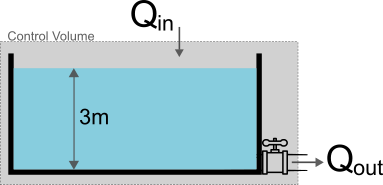
\includegraphics{https://github.com/gregjewi/CambridgeCoaching/raw/master/InitialValueWordProblems/Pool_ControlVolume_IVP.png}
\caption{Control Volume Diagram}
\end{figure}

    \hypertarget{formulate-the-question-as-math}{%
\subsection{3. Formulate the question as
math}\label{formulate-the-question-as-math}}

By writing out all of our given information and drawing a picture we
have a great idea of the relationship we may be looking for: the water
height as a function of time, or \(h(t)\).

But remember, the question actually asks how much time the job will take
or, \(t_{total}\). We know the parts of \(t_{total}\) are:
\[t_{total} = t_{drive} + t_{drain} + t_{repair}\]

Plugging in the known times, \(t_{drive}\) and \(t_{repair}\), we have:

\[t_{total} = 6 + t_{drain}\]

The time needed to drain the pool is the time between when the drain is
opened, and the pool meets our initial conditions \(h_{pool}(t_0) = 2\),
and when the depth of water in the pools is zero,
\(h_{pool}(t \,= \, ?) = 0\).

    \hypertarget{make-a-differential-relationship}{%
\subsection{4. Make a differential
relationship}\label{make-a-differential-relationship}}

We know we want the end result to be of the form \(h(t)\). Where to
start? For Control Volume problems it is almost always automatic to
write down the following equation:

\[\Delta V = \left(Q_{in} - Q_{out}\right) \cdot \Delta t\]

Where \(\Delta V\) is the change of stuff within the Control Volume's
(ie. water in the the pool,) and \(Q_{in}\), \(Q_{out}\) are volumetric
rates of stuff going into and out of the control volume (ie. water going
into and out of the pool,) during a discrete slice of time,
\(\Delta t\). Does this make sense? Yes! \textbf{Just check the units.}

\[\left[m^3\right] = \left[\frac{m^3}{hr}\right] \cdot \left[hr\right]\]

Making sure the units check out for applied calculus is always a great
sanity check.

So the units check out, let's break down the pieces of this equation. On
left, because the footprint of the pool is constant at every height,
always \(5 \times 10 \, m\), the only dimension that changes with a
change in volume is height, or

\[\Delta V_{pool} = A_{pool} \cdot \Delta h\]

On the right, there is nothing going into the pool so \(Q_{in}\) is
zero. \(Q_{out}\) we are given as the orifice equation. Plugging these
values in, we have

\[\Delta V_{pool} = \left(0 - C_d \sqrt{h} \right) \cdot \Delta t\]
\[\Delta V_{pool} = - C_d \sqrt{h} \, \Delta t\]

Combining these we get

\[A_{pool} \cdot \Delta h = - C_d \sqrt{h} \, \Delta t\]

Collecting the \(h\) terms on one side and taking the differentials
\(\Delta h\) and \(\Delta t\) to their infinitesimal limits \(d h\) an
\(d t\),

\[A_{pool} \cdot dh = - C_d \sqrt{h} \, dt\]
\[- h^{-1/2} dh = \frac{C_d}{A_{pool}} \, dt\]

    \hypertarget{solve-the-integral-plug-in-initial-condition}{%
\subsection{5. Solve the Integral, Plug in Initial
Condition}\label{solve-the-integral-plug-in-initial-condition}}

Congrats, \textbf{the hard part is done!} You've successfully arranged
the block of text into familiar equations to be integrated. All that
remains is to solve the integral and plug in our initial condition.
Let's go:

\[\int - h^{-1/2} dh = \int \frac{C_d}{A_{pool}} \, dt\]
\[-2 \sqrt{h} + k_1 = \int \frac{C_d}{A_{pool}} \, dt\]
\[-2 \sqrt{h} + k_1 = \frac{C_d}{A_{pool}} \, t + k_2\]

Combining the constants and rearranging, we get

\[\sqrt{h} = K - \frac{C_d}{2 \, A_{pool}} \cdot t\]

Using our initial condition, \(h(t_0) = 3\), we can solve for \(K\),

\[\sqrt{3} = K - \frac{C_d}{2 \, A_{pool}} \cdot 0\] \[\sqrt{3} = K\]

Thus, \[\sqrt{h} = \sqrt{3} - \frac{C_d}{2 \, A_{pool}} \cdot t\]

At this point we \emph{could} continue to organize the equation, ie.
square each side and have something in the form of \(h(t)\). But, you'll
notice that we don't need to organize any further to answer our
question: find the time, \(t_{drain}\), when \(h = 0\).

    \hypertarget{answer-the-question}{%
\subsection{6. Answer the Question}\label{answer-the-question}}

We've got our relationship between \(h\) and \(t\) that to compute the
following: find the time, \(t_{drain}\), when \(h = 0\). All that is
left is plug in \(h=0\) and solve for \(t_{drain}\).

\[\sqrt{0} = \sqrt{3} - \frac{C_d}{2 \, A_{pool}} \cdot t_{drain}\]
\[t_{drain} = \sqrt{3} \cdot \frac{2 \, A_{pool}}{C_d}\]
\[t_{drain} = \sqrt{3} \cdot \frac{2 \cdot 50}{180}\]
\[t_{drain} = 0.96 \, hr \approx 1 \, hr\]

So,

\[t_{total} = 6 + t_{drain}\] \[\boxed{t_{total} = 7 \, hr}\]

    And there you have it. All in a day's work.

    \textbf{Extra Credit:} The Python code below shows how to plot the
height of the water in the pool between time {[}0,1{]}.

    \begin{Verbatim}[commandchars=\\\{\}]
{\color{incolor}In [{\color{incolor}53}]:} \PY{c+c1}{\PYZsh{} Import packages}
         \PY{k+kn}{import} \PY{n+nn}{matplotlib}\PY{n+nn}{.}\PY{n+nn}{pyplot} \PY{k}{as} \PY{n+nn}{plt}
         \PY{k+kn}{import} \PY{n+nn}{numpy} \PY{k}{as} \PY{n+nn}{np}
\end{Verbatim}


    \begin{Verbatim}[commandchars=\\\{\}]
{\color{incolor}In [{\color{incolor}54}]:} \PY{k}{def} \PY{n+nf}{h\PYZus{}of\PYZus{}t}\PY{p}{(}\PY{n}{t}\PY{p}{)}\PY{p}{:}
             \PY{c+c1}{\PYZsh{} Return height of pool given time}
             
             \PY{n}{C\PYZus{}d} \PY{o}{=} \PY{l+m+mi}{180}
             \PY{n}{A\PYZus{}pool} \PY{o}{=} \PY{l+m+mi}{5} \PY{o}{*} \PY{l+m+mi}{10}
             \PY{n}{h\PYZus{}0} \PY{o}{=} \PY{l+m+mi}{3}
             
             \PY{k}{return} \PY{p}{(}\PY{n}{np}\PY{o}{.}\PY{n}{sqrt}\PY{p}{(}\PY{n}{h\PYZus{}0}\PY{p}{)} \PY{o}{\PYZhy{}} \PY{n}{C\PYZus{}d}\PY{o}{/}\PY{p}{(}\PY{l+m+mi}{2} \PY{o}{*} \PY{n}{A\PYZus{}pool}\PY{p}{)} \PY{o}{*} \PY{n}{t}\PY{p}{)}\PY{o}{*}\PY{o}{*}\PY{l+m+mi}{2}
\end{Verbatim}


    \begin{Verbatim}[commandchars=\\\{\}]
{\color{incolor}In [{\color{incolor}56}]:} \PY{c+c1}{\PYZsh{} Generate time values on which to evaulate h }
         \PY{n}{t} \PY{o}{=} \PY{n}{np}\PY{o}{.}\PY{n}{arange}\PY{p}{(}\PY{l+m+mi}{0}\PY{p}{,}\PY{l+m+mi}{1}\PY{p}{,}\PY{l+m+mf}{0.01}\PY{p}{)}
         
         \PY{c+c1}{\PYZsh{} Use the map function to evaluate h at all t provided}
         \PY{c+c1}{\PYZsh{} convert to list for plotting}
         \PY{n}{h} \PY{o}{=} \PY{n+nb}{list}\PY{p}{(}\PY{n+nb}{map}\PY{p}{(}\PY{n}{h\PYZus{}of\PYZus{}t}\PY{p}{,}\PY{n}{t}\PY{p}{)}\PY{p}{)}
\end{Verbatim}


    \begin{Verbatim}[commandchars=\\\{\}]
{\color{incolor}In [{\color{incolor}58}]:} \PY{c+c1}{\PYZsh{} Make a pretty plot.}
         \PY{n}{plt}\PY{o}{.}\PY{n}{figure}\PY{p}{(}\PY{n}{figsize}\PY{o}{=}\PY{p}{(}\PY{l+m+mi}{8}\PY{p}{,}\PY{l+m+mi}{6}\PY{p}{)}\PY{p}{)}
         \PY{n}{plt}\PY{o}{.}\PY{n}{plot}\PY{p}{(}\PY{n}{t}\PY{p}{,}\PY{n}{h}\PY{p}{,}\PY{n}{color}\PY{o}{=}\PY{l+s+s1}{\PYZsq{}}\PY{l+s+s1}{grey}\PY{l+s+s1}{\PYZsq{}}\PY{p}{,}\PY{n}{linestyle}\PY{o}{=}\PY{l+s+s1}{\PYZsq{}}\PY{l+s+s1}{\PYZhy{}\PYZhy{}}\PY{l+s+s1}{\PYZsq{}}\PY{p}{)}
         \PY{n}{plt}\PY{o}{.}\PY{n}{xlabel}\PY{p}{(}\PY{l+s+s1}{\PYZsq{}}\PY{l+s+s1}{Time [hr]}\PY{l+s+s1}{\PYZsq{}}\PY{p}{)}
         \PY{n}{plt}\PY{o}{.}\PY{n}{ylabel}\PY{p}{(}\PY{l+s+s1}{\PYZsq{}}\PY{l+s+s1}{Height of Water in Pool [m]}\PY{l+s+s1}{\PYZsq{}}\PY{p}{)}
         \PY{n}{plt}\PY{o}{.}\PY{n}{title}\PY{p}{(}\PY{l+s+s1}{\PYZsq{}}\PY{l+s+s1}{Water Height vs. Time}\PY{l+s+s1}{\PYZsq{}}\PY{p}{)}
         \PY{n}{plt}\PY{o}{.}\PY{n}{xticks}\PY{p}{(}\PY{p}{[}\PY{l+m+mi}{0}\PY{p}{,}\PY{l+m+mf}{0.5}\PY{p}{,}\PY{l+m+mi}{1}\PY{p}{]}\PY{p}{)}
         \PY{n}{plt}\PY{o}{.}\PY{n}{yticks}\PY{p}{(}\PY{p}{[}\PY{l+m+mi}{0}\PY{p}{,}\PY{l+m+mf}{1.5}\PY{p}{,}\PY{l+m+mi}{3}\PY{p}{]}\PY{p}{)}
         
         \PY{c+c1}{\PYZsh{} Show the plot.}
         \PY{n}{plt}\PY{o}{.}\PY{n}{show}\PY{p}{(}\PY{p}{)}
\end{Verbatim}


    \begin{center}
    \adjustimage{max size={0.9\linewidth}{0.9\paperheight}}{output_14_0.png}
    \end{center}
    { \hspace*{\fill} \\}
    

    % Add a bibliography block to the postdoc
    
    
    
    \end{document}
